\documentclass[tikz,convert]{standalone}

\usetikzlibrary{decorations.pathreplacing}

\begin{document}
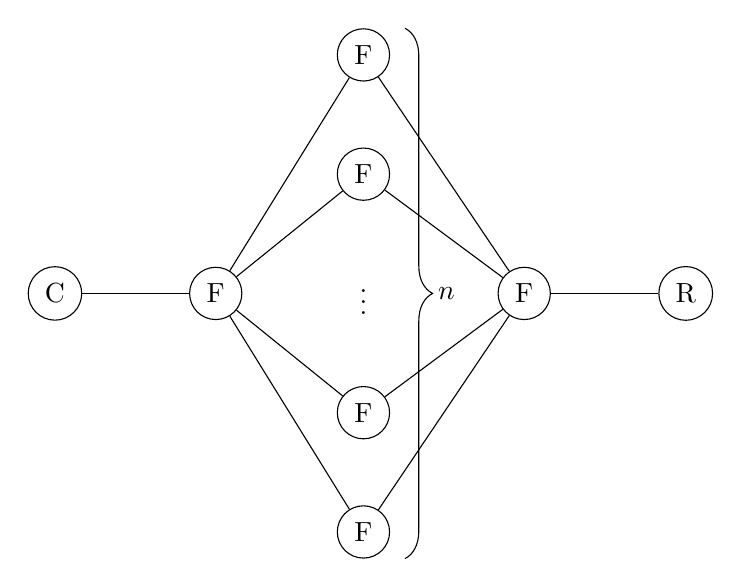
\begin{tikzpicture}
  
  \node[draw, shape=circle] (c) {C};
  \node[draw, shape=circle, right of=c, right=20pt] (fc) {F};
  
  \node[right of=fc, right=20pt] (ellipsis) {\vdots};
  \node[draw, shape=circle, above of=ellipsis, above=5pt] (f2) {F};
  \node[draw, shape=circle, above of=f2, above=5pt] (f1) {F};
  \node[draw, shape=circle, below of=ellipsis, below=5pt] (f3) {F};
  \node[draw, shape=circle, below of=f3, below=5pt] (f4) {F};
  
  \node[draw, shape=circle, right of=ellipsis, right=20pt] (fr) {F};
  \node[draw, shape=circle, right of=fr, right=20pt] (r) {R};

  \path[draw, -] (c) to (fc);
  \path[draw, -] (fr) to (r);
  \path[draw, -] (fc) to (f1);
  \path[draw, -] (fc) to (f2);
  \path[draw, -] (fc) to (f3);
  \path[draw, -] (fc) to (f4);
  \path[draw, -] (fr) to (f1);
  \path[draw, -] (fr) to (f2);
  \path[draw, -] (fr) to (f3);
  \path[draw, -] (fr) to (f4);

  \draw[decorate, decoration={brace, amplitude=10pt}]
  ([xshift=15pt] f1.north) -- ([xshift=15pt] f4.south)
  node [midway, xshift=15pt] {$n$};
  
\end{tikzpicture}
\end{document}
